%%%%%%%%%%%%%%%%%%%%%%%%%%%%%%%%%%%%%%%
%%  MISCELLANEOUS SETTINGS/COMMANDS  %%
%%%%%%%%%%%%%%%%%%%%%%%%%%%%%%%%%%%%%%%


\newcommand{\balA}[1][1]{BAL$^\mathup{I}_{#1:#1}$\xspace}
\newcommand{\unbalA}[1][n]{UNBAL$^\mathup{I}_{1:#1}$\xspace}
\newcommand{\balB}[1][1]{BAL$^\mathup{II}_{#1:#1}$\xspace}
\newcommand{\unbalB}[1][n]{UNBAL$^\mathup{II}_{#1:1}$\xspace}

%% Add separator slide to the beginning of each section ==>
\AtBeginSection[]{
	\begin{frame}[standout, c]{~}
		%\vfill
		\usebeamerfont{title}%
		\textcolor{SpotColor}{\insertsectionhead}
		%\vfill
	\end{frame}%
}

%% Alternativelyy, add ``Outline'' slide to the beginning of each section ==>
%\AtBeginSection[]{
%	\begin{frame}[plain]{Outline}
%		\tableofcontents[currentsection]
%	\end{frame}
%}
%% <==

\title{A~Template for Academic Presentations}
%\subtitle{}

\author[Smith, Smith, and Smith]{%
	Adam Smith\inst{a,\,c} \and
	% Set the name of the presenting coauthor in boldface:
	\alert{Janet Smith}\inst{b,\,c} \and
	Jeremiah Smith\inst{a}
} % Author(s)

\institute{%
	\\
	\inst{a}\,University of Bonn, Germany \and
	\inst{b}\,University of Cologne, Germany \and
	\inst{c}\,Collaborative Research Center Transregio~224%
} % Institution(s)

\date{%
	\\
	Name of the Inviting Institution/Seminar Series \\[\medskipamount]
	\textmd{\today}%
}




%%%%%%%%%%%%%%%%%%%
%%  TITLE SLIDE  %%
%%%%%%%%%%%%%%%%%%%


\begin{frame}[standout]{~}

	\Wider{%
		\titlepage%
	}

\end{frame}



\begin{frame}[standout]{Outline}

	\medskip
	\tableofcontents

\end{frame}




%%%%%%%%%%%%%%%%%
%%  MAIN PART  %%
%%%%%%%%%%%%%%%%%


\section{Introduction}


\begin{frame}{\titleprefix}

	\heading{Background}
	\begin{itemize}
		\item Temporal discounting is key concept in economics.
		\item Normative model: exponential discounting. However, observed decisions are hard to explain \citep[e.g.,][]{Dohmen2012}.
		\item One alternative: the ``focusing model'' by \cite{Koszegi2013}.
	\end{itemize}
	
	\heading{Research Question}
	\begin{itemize}
		\item The composition of latex and of typical rubbers is given below.
		\item Is it true that trees are regularly tapped and the coagulated latex which exudes is collected and worked up into rubber?
	\end{itemize}

\end{frame}


\begin{frame}{\titleprefix}

	\heading{Preview of the Results}
	\begin{itemize}
		\item There is no feasible method at present known of preventing the inclusion of the resin of the latex with the rubber during coagulation.
		\item[$\Rightarrow$] Although the separation of the resin from the solid caoutchouc by means of solvents is possible, it is not practicable or profitable commercially.
	\end{itemize}

\end{frame}


\section{Study Design}


\begin{frame}{\titleprefix: Design of the Study}

	\begin{quote}
		Great Minds Discuss Ideas. \\
		Average Minds Discuss Events. \\
		Small Minds Discuss People. \\
		\upshape ---\url{https://quoteinvestigator.com/2014/11/18/great-minds/}
	\end{quote}

	\begin{itemize}
		\item The latex of the best rubber plants furnishes from 20\% to 50\% of rubber.
		\item As the removal of the impurities of the latex is one of the essential points to be aimed at, it was thought that the use of a centrifugal machine to separate the caoutchouc as a cream from the watery part of the latex would prove to be a satisfactory process.
	\end{itemize}

\end{frame}


\begin{frame}{\titleprefix: Design of the Study}

	The watery portion of the latex soaks into the trunk, and the soft spongy rubber which remains is kneaded and pressed into lumps or balls:
	
	\alert{\balA, \balB:} Each payment transferred on single day.
	
	\alert{\unbalA:} Earlier payoff concentrated, while later payoff dispersed over ${n = 2}$, 4, or 8~dates.
	
	\alert{\unbalB:} Earlier payoff dispersed over ${n = 2}$, 4, or 8 dates, while later payoff concentrated.

\end{frame}


\begin{frame}{\titleprefix: Control Experiment}

	\begin{itemize}
		\item Control for alternative explanations.
		\item Many of the example sentences were taken from \url{http://sentence.yourdictionary.com/latex}.
	\end{itemize}

\end{frame}


\begin{frame}{\titleprefix: An~Example \texttt{enumerate} List}

	\blindlistlist[3]{enumerate}[4]

\end{frame}


\begin{frame}{\titleprefix: An~Example \texttt{itemize} List}

	\blindlistlist[3]{itemize}[4]

\end{frame}


\begin{frame}{\titleprefix: Some Example Text}

	\heading{Let's include some Greek letters: $\alpha$, $\beta$}

	\blindtext

\end{frame}


\begin{frame}{\titleprefix: Some Example Formulas}

	\heading{Let's include some additional Greek letters: $\gamma$, $\phi$}
	\[
		p(R, \phi) \sim
			\int_{-\infty}^\infty
				\frac
					{ \tilde{W}_n(\gamma) \exp \left[ \imath R / a \left( \sqrt{k^2 a^2 - \gamma^2} \cos \phi \right) \right] }
					{ (k^2 a^2 - \gamma^2)^{3/4} {H'}_n^{(1)} \left( \sqrt{k^2 a^2 - \gamma^2} \right) }
			\mathup{d}\gamma
	\]
	
	\heading{Let's also include some upright Latin letters: $\mathup{d}$, $\mathup{e}$}
	\[
		\int_{a}^{b} f(x)\,\mathup{d}x = F(b) - F(a)
	\]

\end{frame}


\begin{frame}{\titleprefix: Additional Example Formulas (with upright $\mathup{\pi}$)}

	\def\Pr{\ensuremath{\mathbb{P}}}
	\def\rmd{\mathup{d}}
	Only variables are set in italics according to \caps{ISO} style---hence, we use upright ``$\rmd$,'' ``$\mathup{e}$,'' and ``$\mathup{\pi}$'' (\texttt{\textbackslash mathup\{d\}}, \texttt{\textbackslash mathup\{e\}}, and \texttt{\textbackslash mathup\{\textbackslash pi\}}, respectively).
	
	\begin{theorem}[Simplest form of the \emph{Central Limit Theorem}]
		\ifnum \serifbodyfont=0
			\sffamily
		\fi
		Let $X_1, X_2, \cdots$ be a sequence of i.i.d. random variables with mean $0$ 
		and variance $1$ on a probability space $(\Omega, \mathcal{F}, \Pr)$. Then
		\[
			\Pr\left(\frac{X_1+\cdots+X_n}{\sqrt{n}}\le y\right) \to \mathfrak{N}(y) \coloneqq 
			\int_{-\infty}^y \frac{\mathup{e}^{-v^2/2}}{\sqrt{2\mathup{\pi}}}\,
			\mathup{d}v\quad\text{as} \quad n\to\infty,
		\]
		or, equivalently, letting $S_n \coloneqq \sum_1^n X_k$,
		\[
			\mathbb{E} f\left(S_n/\sqrt{n}\right)\to \int_{-\infty}^\infty f(v)
			\frac{\mathup{e}^{-v^2/2}}{\sqrt{2\piup}}\,\mathup{d}v
			\quad\mbox{as $n\to\infty$, for every $f\in\mathup{b}
			\mathcal{C}(\mathbb{R})$.}
		\]
	\end{theorem}

\end{frame}


\section{Results}


\begin{frame}{\titleprefix: Overview}

	\begin{enumerate}
		\item As a secondary function we may recognize the power of closing wounds, which results from the rapid coagulation of exuded latex in contact with the air:
		\begin{enumerate}
			\item In some cases (Allium, Convolvulaceae, etc.) rows of cells with latex-like contents occur.
			\item However, the walls separating the individual cells do not break down.
		\end{enumerate}
		\item The rows of cells from which the laticiferous vessels are formed can be distinguished (6.3~p.p. vs. 2.6~p.p.; ${p < 0.01}$).
	\end{enumerate}

\end{frame}


\begin{frame}{\titleprefix: Our Main Results}

	The charts are taken from \cite{Dertwinkel-Kalt2017}.
	
	(A)~Difference between treatment and control condition.\\
	(B)~Heterogeneity.
	
	\bigskip
	
	\begin{minipage}[t]{\textwidth}
		\begin{minipage}[t]{0.46\textwidth}
			\Large\textbf{A} \textcolor{SpotColor}{\hspace{0.375in} {\small \textbf{Result~1}}} \\[15pt]
			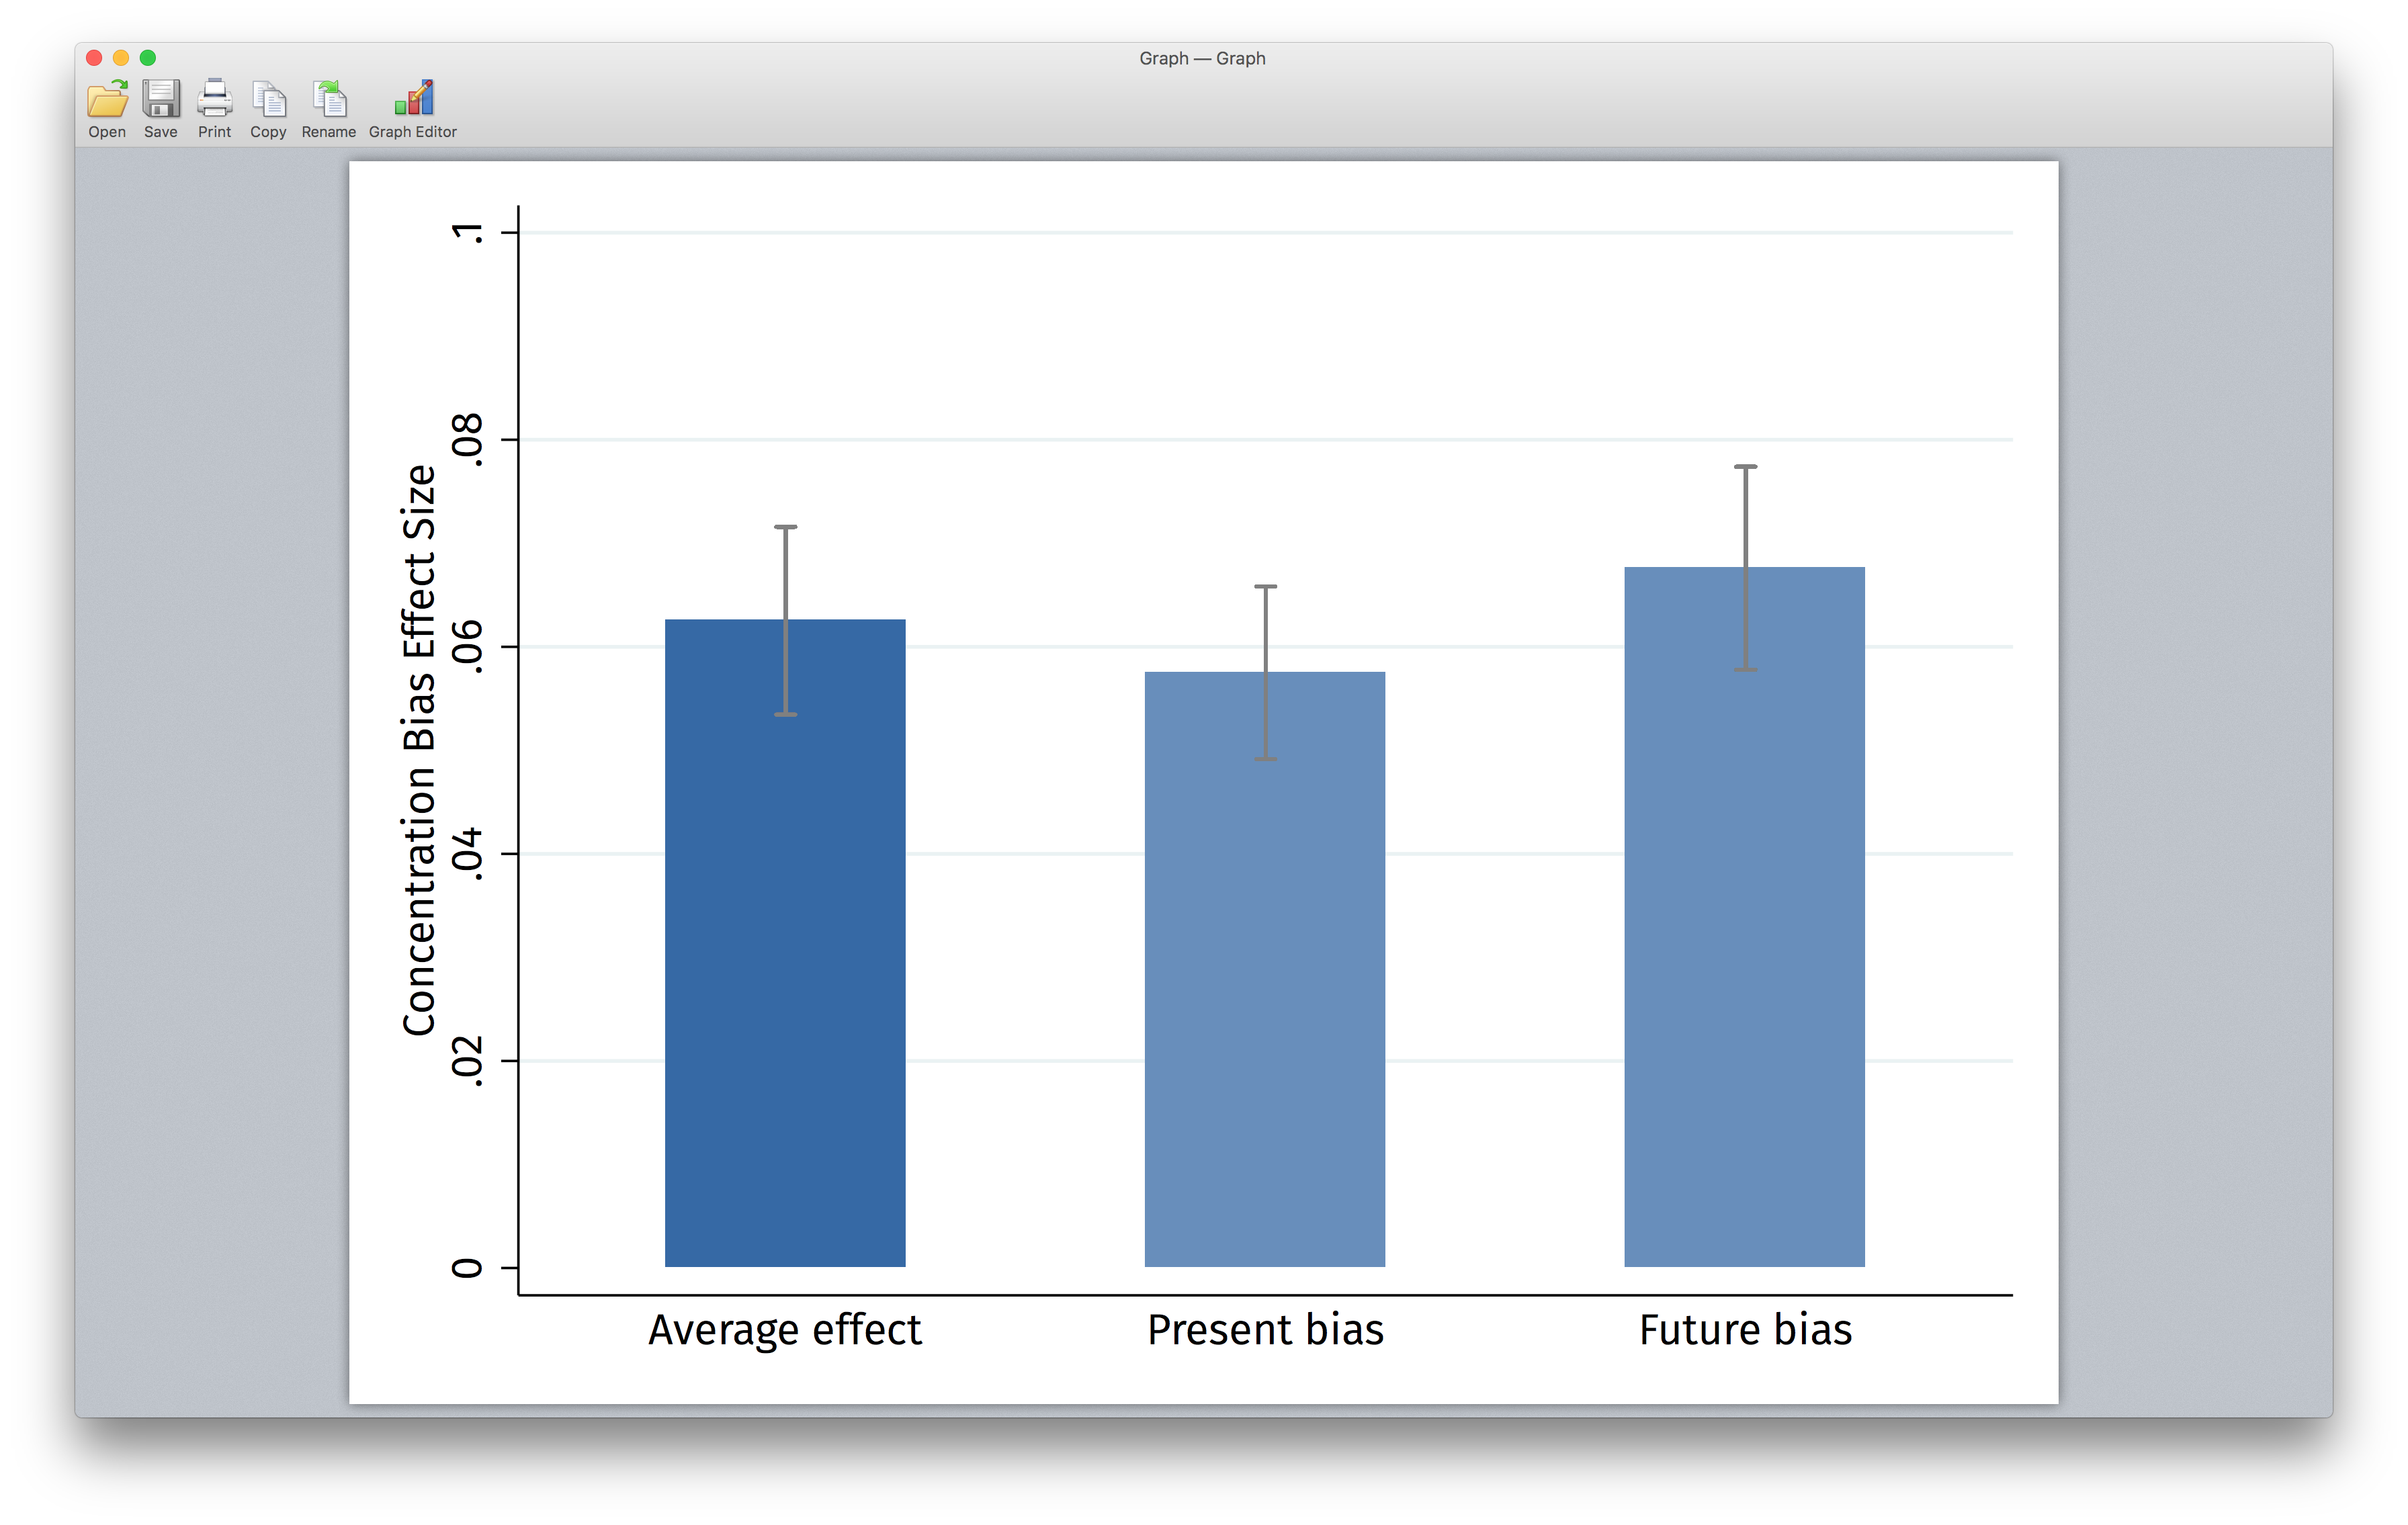
\includegraphics[width=1.643in, trim={3.75in 1.75in 3.75in 2in}, clip]
				{1_Example_Content/Images/average_pb_fb.png} \\
			\centering \footnotesize \sffamily
			$\text{\balA} - \text{\unbalA[\bullet]}$
		\end{minipage}
		\hspace{2pt}
		\begin{minipage}[t]{0.46\textwidth}
			\Large\textbf{B} \textcolor{SpotColor}{\hspace{0.39in} {\small \textbf{Result~2}}} \\[15pt]
			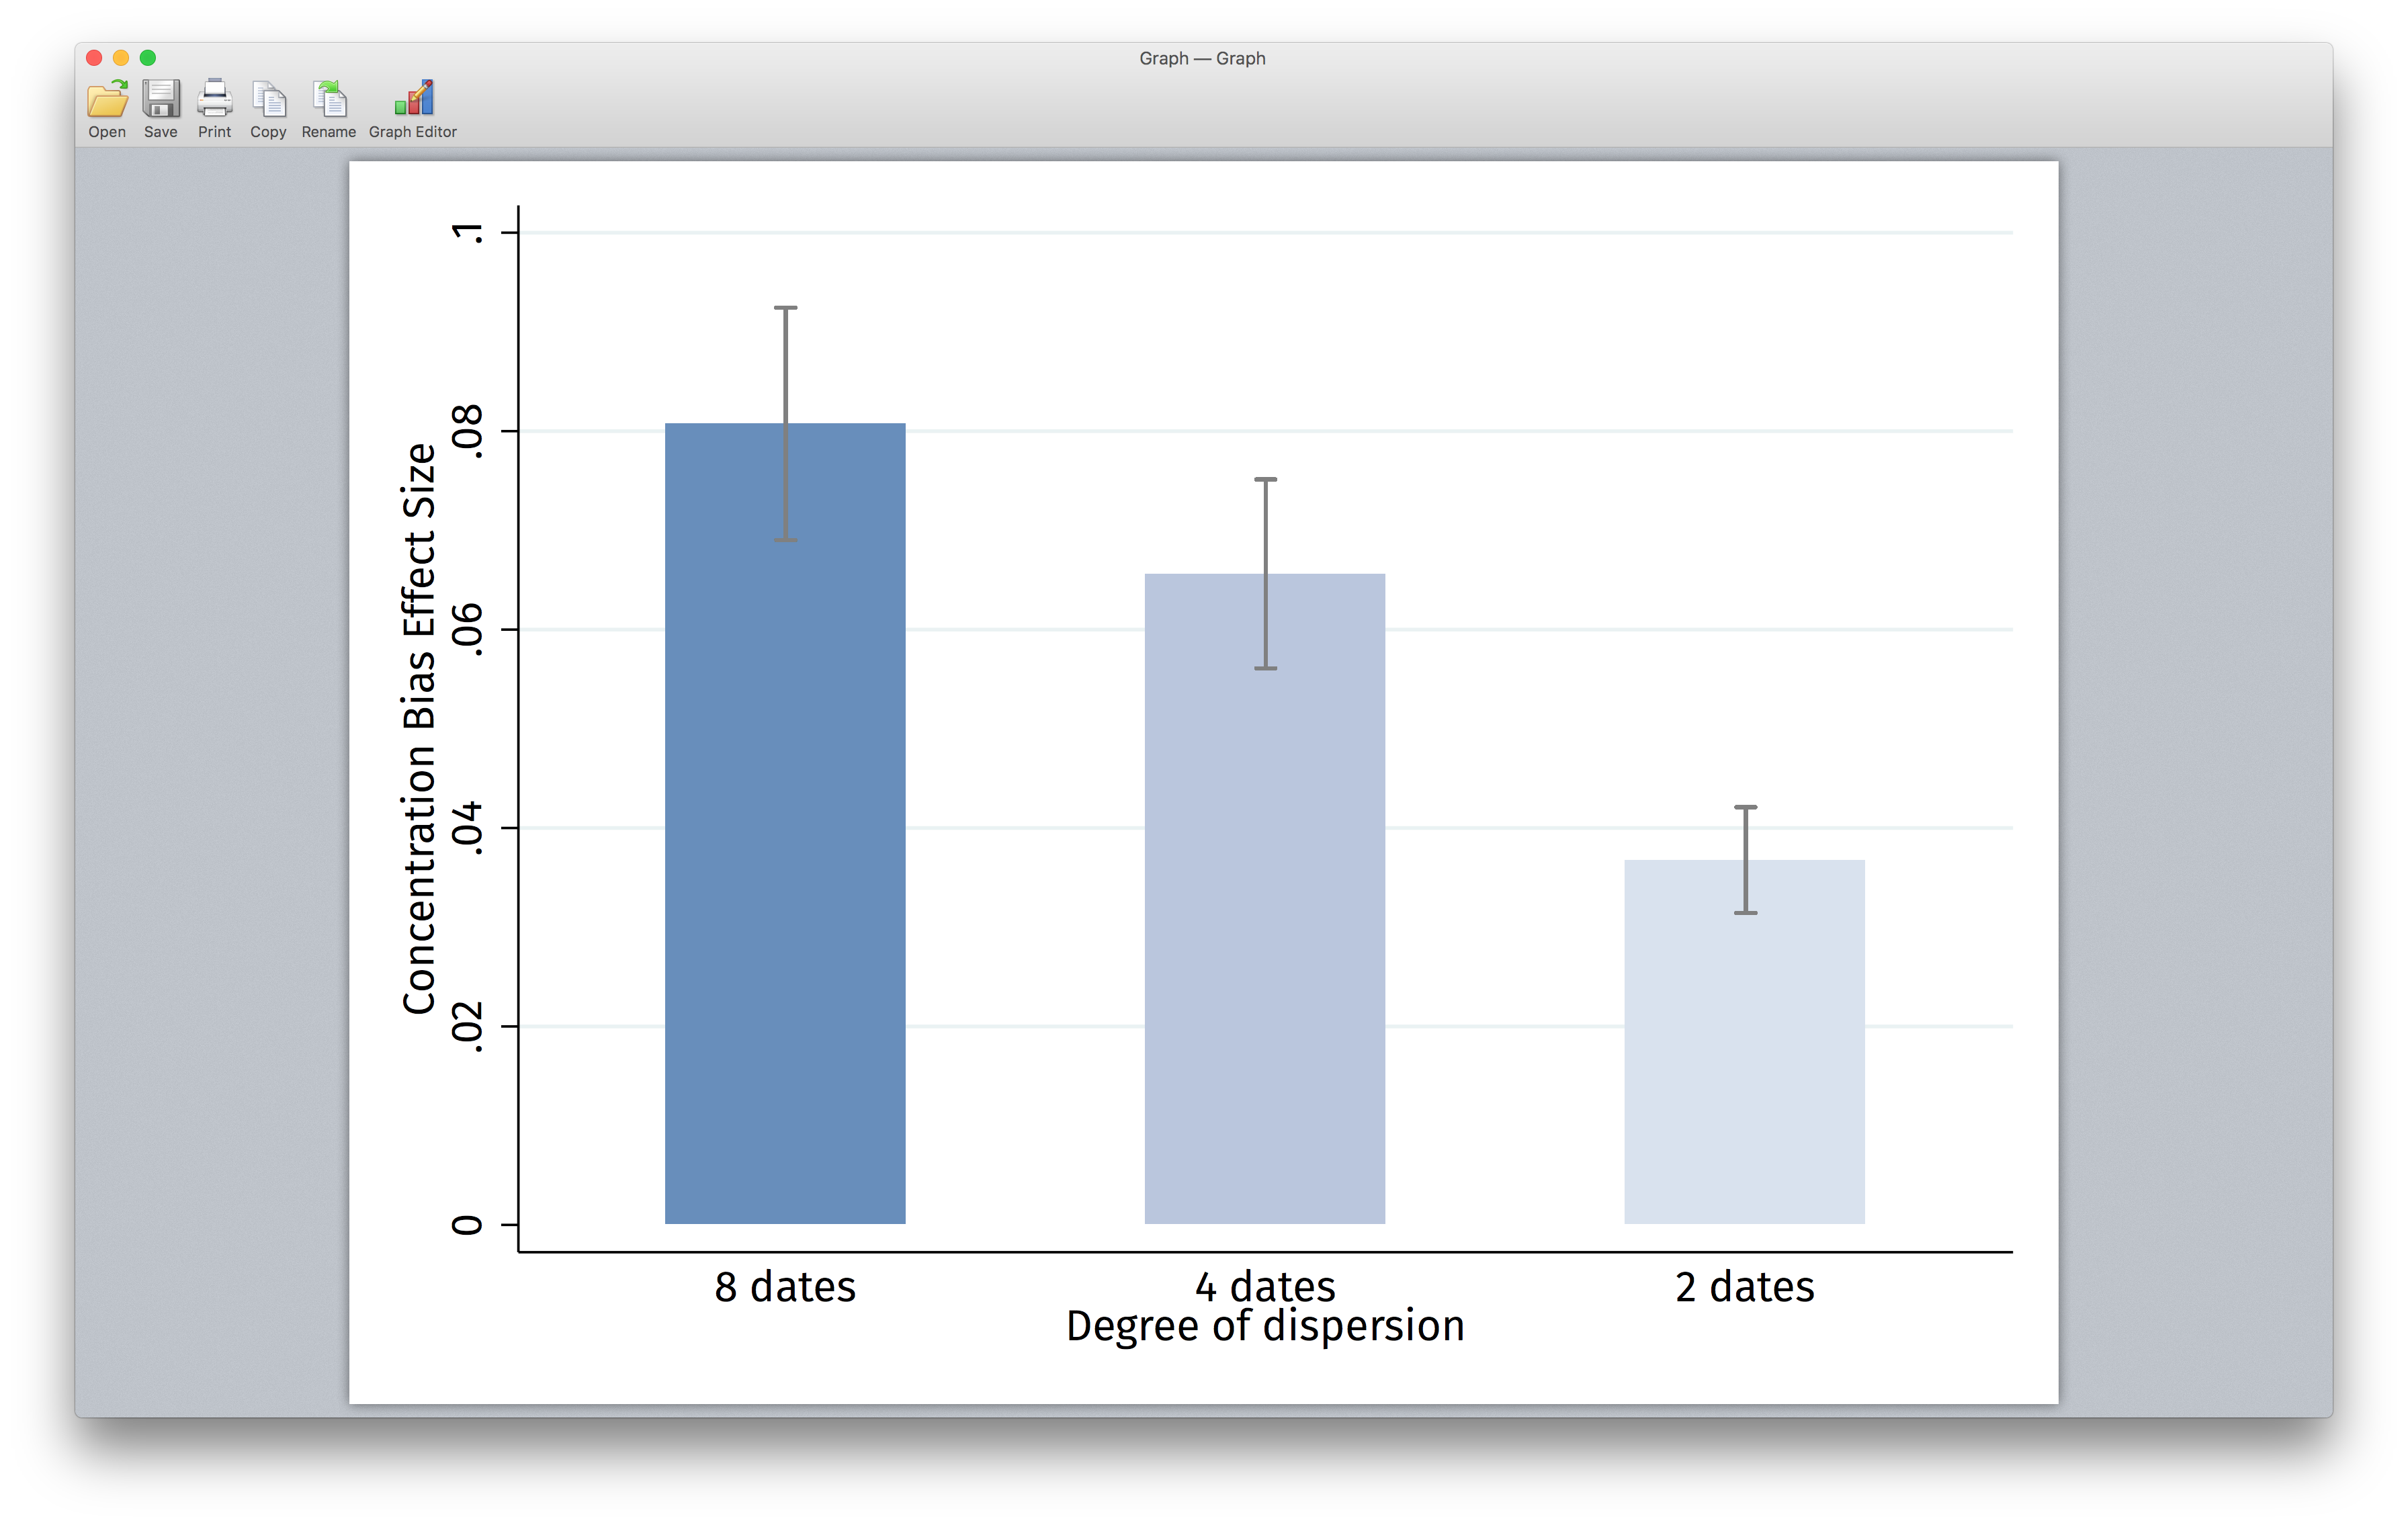
\includegraphics[width=1.710in, trim={3.75in 1.75in 3.75in 2in}, clip]
				{1_Example_Content/Images/average_8_4_2.png} \\
			\centering \footnotesize \sffamily
			$\text{\unbalB[\bullet]} - \text{\balB}$
		\end{minipage} \\
	\end{minipage}
	
\end{frame}


\begin{frame}{\titleprefix: Main vs. Control Experiment}

	Rule out some alternative explanations.
	
	\bigskip
	
	\centering
	{\small \alert{Result~3}} \\[15pt]
	% trim={<left> <lower> <right> <upper>}
	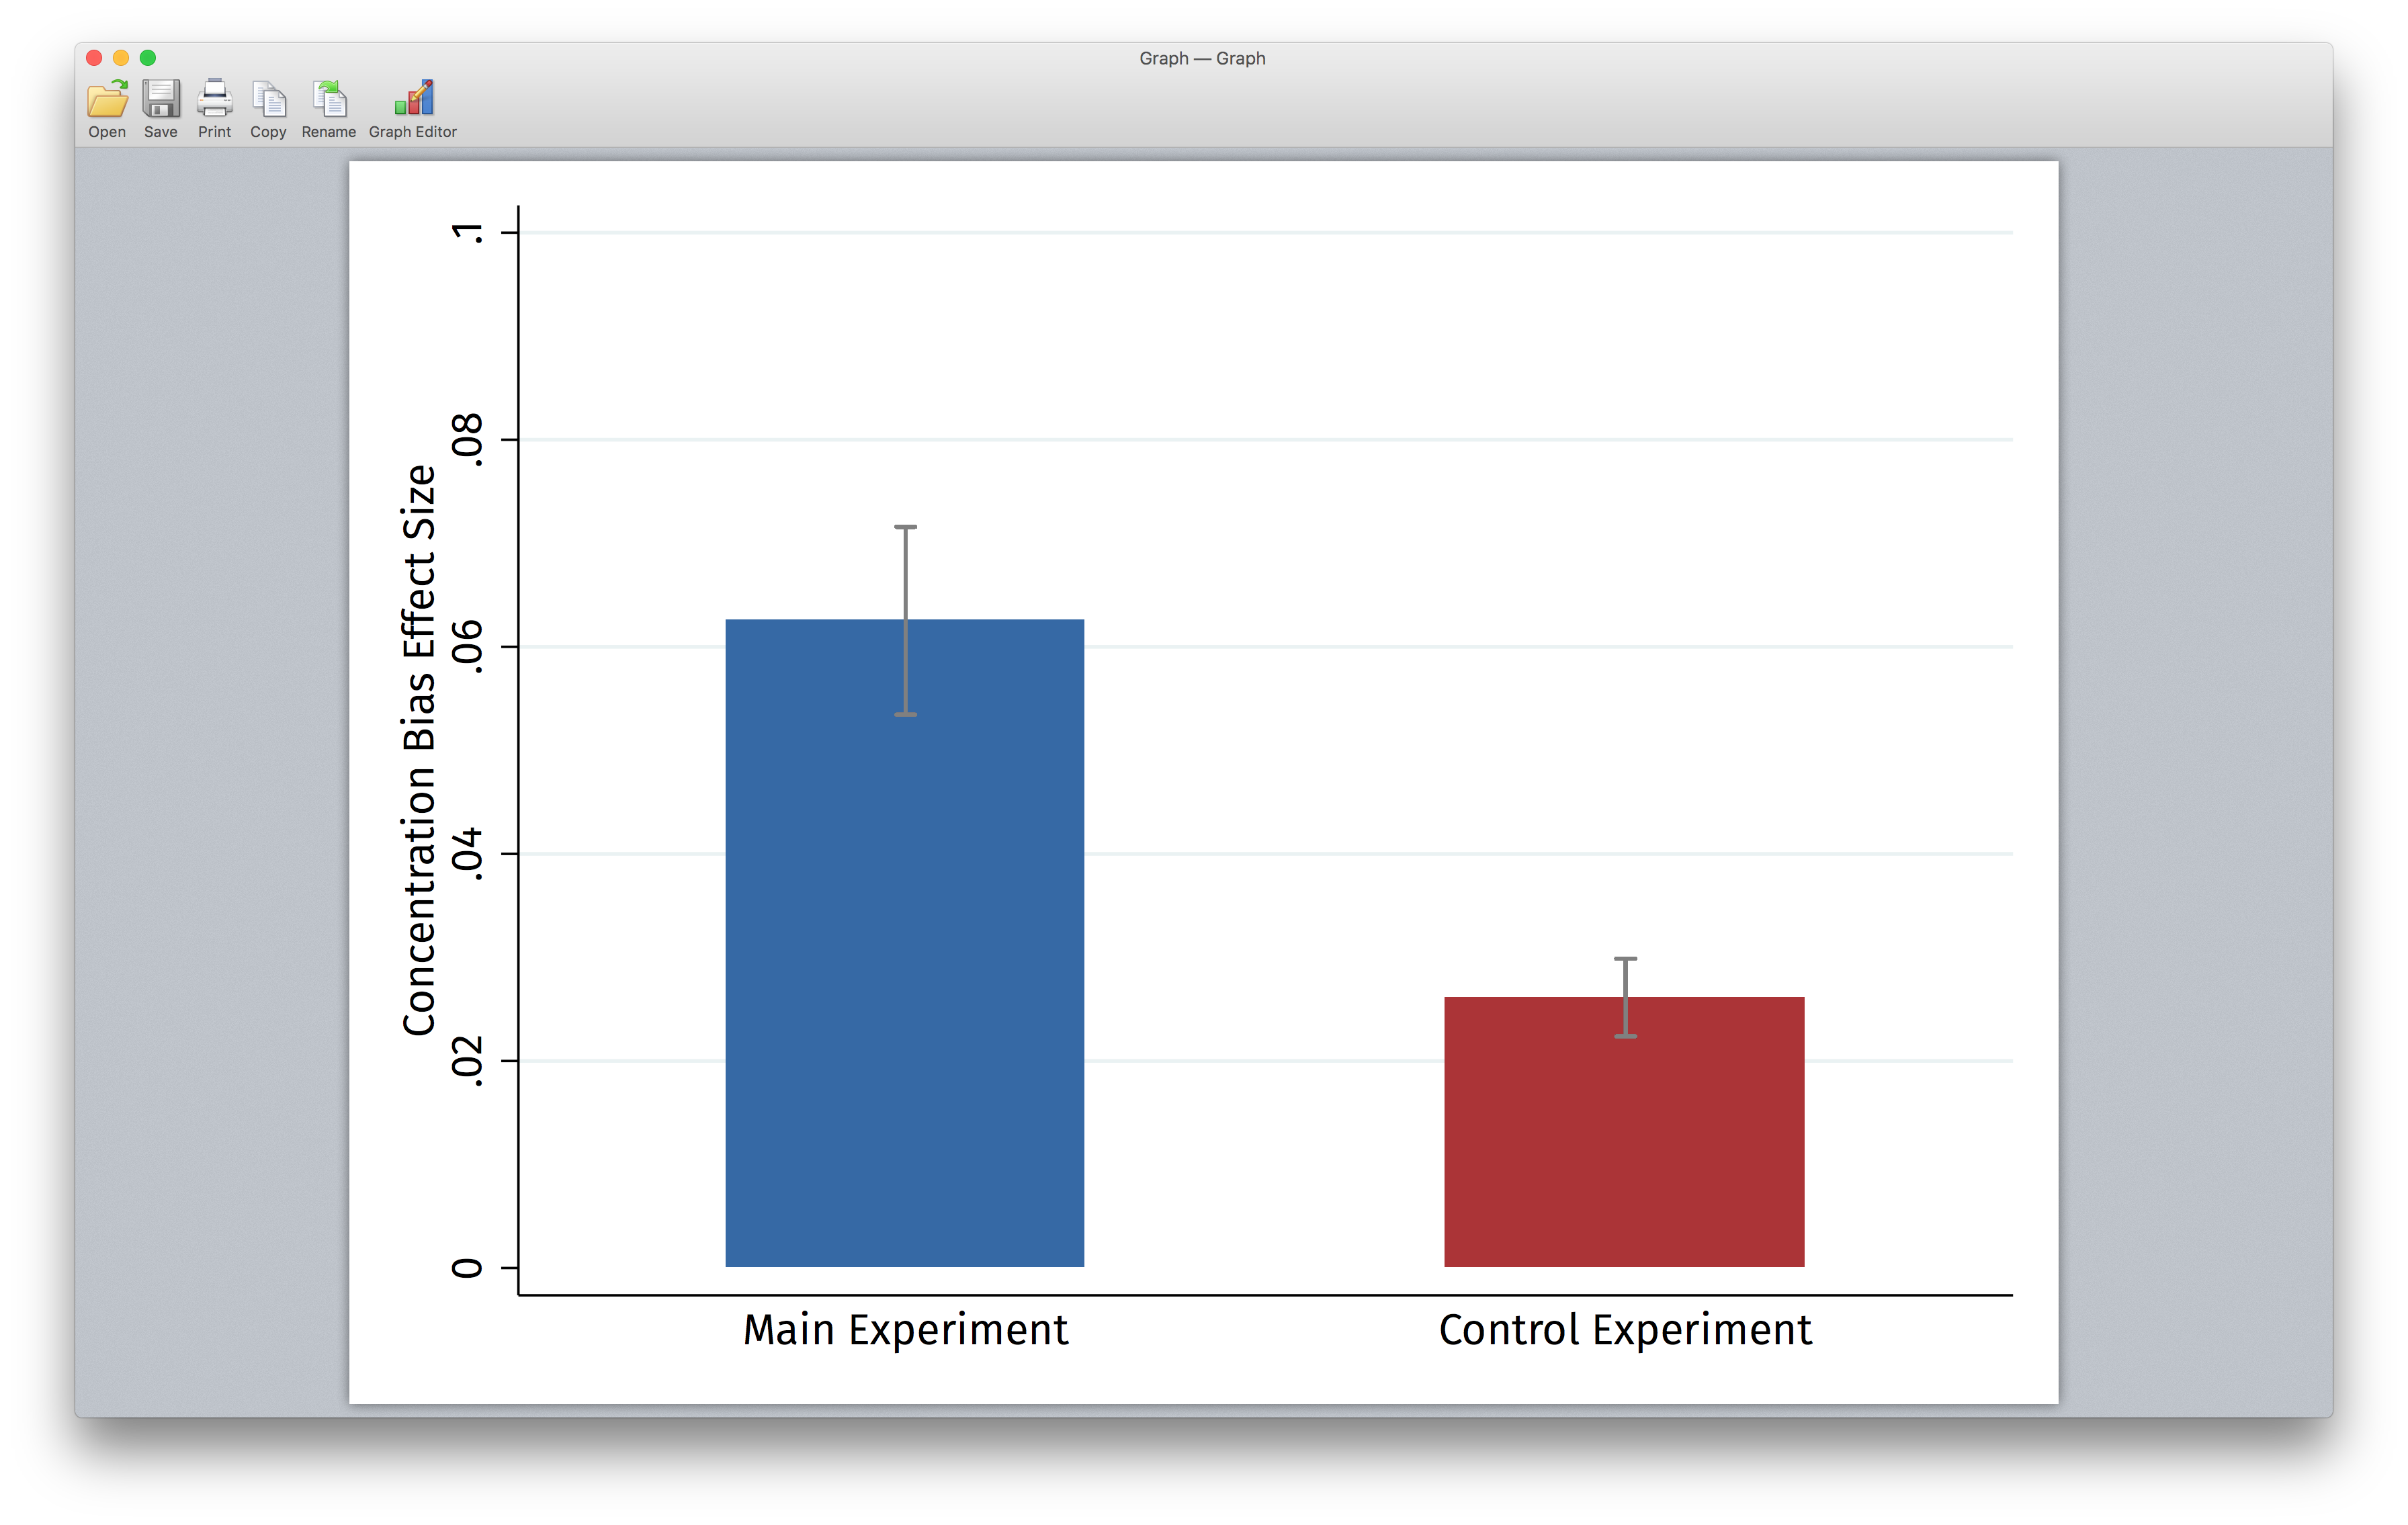
\includegraphics[height=0.5\textheight, trim={3.75in 1.75in 3.75in 2in}, clip]
		{1_Example_Content/Images/average_main_control.png}

\end{frame}


\section{Discussion}


\begin{frame}{\titleprefix}

	\begin{itemize}
		\item The latex exhibits a neutral, acid, or alkaline reaction, depending on the plant from which it was obtained.
		\item The latex is therefore usually allowed to coagulate on the tree \citep{Koszegi2013}.
			\begin{itemize}
				\item[$\Rightarrow$] The latex, which is usually coagulated by standing or by heating, is obtained from incisions.
			\end{itemize}
		\item See also \cite{Bordalo2013}.
	\end{itemize}	

\end{frame}


\begin{frame}{\titleprefix: Conclusion}

	\begin{itemize}
		\item When exposed to air, the latex gradually undergoes putrefactive changes accompanied by coagulation.
		\item The addition of a small quantity of ammonia or of formalin to some latices has the effect of preserving them.
		\item There is, however, reason to believe the following.
		\item The coagulation of latex into rubber is not mainly of this character.
	\end{itemize}

\end{frame}


\begin{frame}{\titleprefix: An Automated Animation}

The automated transition to the next slide (=~page in the PDF document) only works in full-screen mode.
\begin{itemize}
	\item The feature is available in Adobe Acrobat and Acrobat Reader.
	\item Unfortunately, it is (currently, \today) not available in macOS Preview, Skim, and SumatraPDF.
\end{itemize}

\medskip

\transduration{0.25}%
\only<12>{\transduration{}}\hypertarget<1>{animation_start}{}%
\foreach \n [evaluate=\n as \angle using \n * 30] in {0, ..., 12}{
	\only<\n>{
		\begin{figure}
			\begin{tikzpicture}
				\draw[draw=none, use as bounding box](-1, 0) rectangle (1, 2);
				\filldraw[fill=SpotColor, draw=none] (0,1) -- (0,2) arc (90:90-\angle:1cm) -- cycle;
			\end{tikzpicture}
			\caption{Step~\n---Angle: \angle\textdegree}
		\end{figure}
	}
}%
\hyperlink<12>{animation_start}{\beamerreturnbutton{Back to the start}}
		
\end{frame}




%%%%%%%%%%%%%%%%%%
%%  REFERENCES  %%
%%%%%%%%%%%%%%%%%%


\section{\refname}


\begin{frame}[allowframebreaks]{\insertsection}
	
	\bibliographystyle{0_0_Preamble/aea_doi_url_href}
	\bibliography{Library}
	
\end{frame}




%%%%%%%%%%%%%%%%
%%  APPENDIX  %%
%%%%%%%%%%%%%%%%


\begin{appendix}


\section[Appendix \\ \textmd{Backup Slides}]{Appendix}


\begin{frame}[label=model]

	\frametitle{\insertsection: Modeling Concentration Bias}
	
	Subjects consider a sequences of consequences $\boldsymbol{c}$ from choice set $\boldsymbol{C}$.
	
	%Focusing theory augments discounted utility (constant, hyperbolic, \dots) through an~additional weight \highlight{$g[\cdot]$} on the instantaneous utility function.
	\begin{itemize}
	
	\item \alert{Standard discounted utility:}
		Suppose that the instantaneous utility function $u$ satisfies ${u'>0}$ and ${u''\leq 0}$, and that earlier consequences are preferred over later consequences of the same magnitude, i.e., ${D(t)\leq 1}$:
	\item[] ${U}(\boldsymbol{c}\phantom{, \boldsymbol{C}}) \coloneqq
		\sum_{t=1}^{T} \phantom{g_t} D(t)\,u(c_t)$, \quad where, e.g., \quad $D(t) = \delta^t$  or $D(t) = \frac{1}{1 + k\,t}$. %$\beta \delta^t$.
	\medskip
	\item \only<1->{\alert{Focusing model \citep{Koszegi2013}:}}
	\item[]<1-> $\tilde{U}(\boldsymbol{c}, \boldsymbol{C}) \coloneqq \sum_{t=1}^{T} \highlight{g_t}\,D(t)\,u(c_t)$, \quad where \\[3pt]
		\highlight{$g_t \equiv % g[\Delta_t(C)]$, $\Delta_t(C) =
		g[\max_{\boldsymbol{c}'\in \boldsymbol{C}} %D(t) 
		u(c'_t) - \min_{\boldsymbol{c}'\in \boldsymbol{C}} %D(t) 
		u(c'_t)]$}
		\smallskip
		\begin{itemize}
			\item<1-> Weighting function \highlight{$g[\cdot]$} increases in difference of maximum and minimum possible utility at a~point in time.
			\item<1-> Subjects overweight intertemporal consequences with a greater range.
			%\item<3-> Subjects overweight intertemporal consequences with a greater range 
		\end{itemize}
	\end{itemize}

\end{frame}


\end{appendix}